%!Mode:: "TeX:UTF-8"
\documentclass[a4paper,11pt,UTF8]{ctexart}
\usepackage{indentfirst} %缩进
\usepackage{xeCJK}    %使用系统字体
\usepackage{fancyhdr} %自定义页眉页脚
\pagestyle{empty}                   %不设置页眉页脚
\usepackage{amsmath, amsthm, amssymb, amsfonts} %数学公式
\usepackage[a4paper,left=3cm,right=3cm,top=3cm,bottom=3cm]{geometry}
%\usepackage[tmargin=1in,bmargin=1in,lmargin=1.25in,rmargin=1.25in]{geometry}.
\usepackage{booktabs} %插入表格
\usepackage[section]{placeins} %避免浮动
\usepackage{listings} %插入代码
\usepackage{ctex}     %中文宏包
\usepackage[svgnames, table]{xcolor} %彩色表格
\usepackage{algorithm}          %伪代码
\usepackage{algorithmicx}
\usepackage{algpseudocode}
\usepackage{algorithm,algpseudocode,float}
\usepackage{lipsum}
\usepackage{enumitem}           %调整列举环境
\usepackage{url}
\usepackage{fontspec,xunicode}
\usepackage{cite}
\defaultfontfeatures{Mapping=tex-text} %如果没有它,会有一些 tex 特殊字符无法正常使用,比如连字符。

\usepackage{graphicx}
\usepackage{subfigure}
\graphicspath{{imgs/}}

%%%%%%%%%%%%%%%%%%%%%%%%%%%%%%%%%%%%%%%%%%%%%%%%%%%%%%%%%%%%%%%%
% 缩进及行间距
%%%%%%%%%%%%%%%%%%%%%%%%%%%%%%%%%%%%%%%%%%%%%%%%%%%%%%%%%%%%%%%%
\setlength{\parindent}{22pt} %重新定义缩进长度
\setlength{\baselineskip}{20pt}  %定义行间距
%\renewcommand{\baselinestretch}{1.1} %定义行间距

%%%%%%%%%%%%%%%%%%%%%%%%%%%%%%%%%%%%%%%%%%%%%%%%%%%%%%%%%%%%%%%%
% 列表设置
%%%%%%%%%%%%%%%%%%%%%%%%%%%%%%%%%%%%%%%%%%%%%%%%%%%%%%%%%%%%%%%%
\setenumerate{fullwidth,itemindent=\parindent,listparindent=\parindent,itemsep=0ex,partopsep=0pt,parsep=0ex}
\setenumerate[2]{label=\alph*),leftmargin=1.5em}  %二级item设置
\setitemize{itemindent=38pt,leftmargin=0pt,itemsep=-0.4ex,listparindent=26pt,partopsep=0pt,parsep=0.5ex,topsep=-0.25ex}
\setdescription{itemindent=38pt,leftmargin=0pt,itemsep=-0.4ex,listparindent=26pt,partopsep=0pt,parsep=0.5ex,topsep=-0.25ex}

%%%%%%%%%%%%%%%%%%%%%%%%%%%%%%%%%%%%%%%%%%%%%%%%%%%%%%%%%%%%%%%%
% 图的标题行间距设置
%%%%%%%%%%%%%%%%%%%%%%%%%%%%%%%%%%%%%%%%%%%%%%%%%%%%%%%%%%%%%%%%
\newcommand{\bottomcaption}{%
\setlength{\abovecaptionskip}{6pt}%
\setlength{\belowcaptionskip}{6pt}%
\caption}


%%%%%%%%%%%%%%%%%%%%%%%%%%%%%%%%%%%%%%%%%%%%%%%%%%%%%%%%%%%%%%%%
% 字体定义
%%%%%%%%%%%%%%%%%%%%%%%%%%%%%%%%%%%%%%%%%%%%%%%%%%%%%%%%%%%%%%%%
\setmainfont{Times New Roman}  %默认英文字体.serif是有衬线字体sans serif无衬线字体
\setmonofont{Consolas}
\setCJKmainfont[ItalicFont={楷体}, BoldFont={黑体}]{宋体}%衬线字体 缺省中文字体为
\setCJKsansfont{黑体}
\punctstyle{hangmobanjiao}
%-----------------------xeCJK下设置中文字体------------------------------%
\setCJKfamilyfont{song}{SimSun}                             %宋体 song
\newcommand{\song}{\CJKfamily{song}}
\setCJKfamilyfont{fs}{FangSong}                      %仿宋  fs
\newcommand{\fs}{\CJKfamily{fs}}
\setCJKfamilyfont{ktgb}{KaiTi}                      %楷体2312 ktgb
\newcommand{\ktgb}{\CJKfamily{ktgb}}
\setCJKfamilyfont{yh}{Microsoft YaHei}                    %微软雅黑 yh
\newcommand{\yh}{\CJKfamily{yh}}
\setCJKfamilyfont{hei}{SimHei}                              %黑体  hei
\newcommand{\hei}{\CJKfamily{hei}}
\setCJKfamilyfont{hwxk}{STXingkai}                                %华文行楷  hwxk
\newcommand{\hwxk}{\CJKfamily{hwxk}}
%------------------------------设置字体大小------------------------%
\newcommand{\shiyanbaogao}{\fontsize{36pt}{\baselineskip}\selectfont}
\newcommand{\chuhao}{\fontsize{42pt}{\baselineskip}\selectfont}     %初号
\newcommand{\xiaochuhao}{\fontsize{36pt}{\baselineskip}\selectfont} %小初号
\newcommand{\yihao}{\fontsize{28pt}{\baselineskip}\selectfont}      %一号
\newcommand{\erhao}{\fontsize{21pt}{\baselineskip}\selectfont}      %二号
\newcommand{\xiaoerhao}{\fontsize{18pt}{\baselineskip}\selectfont}  %小二号
\newcommand{\sanhao}{\fontsize{15.75pt}{\baselineskip}\selectfont}  %三号
\newcommand{\sihao}{\fontsize{14pt}{\baselineskip}\selectfont}       %四号
\newcommand{\xiaosihao}{\fontsize{12pt}{\baselineskip}\selectfont}  %小四号
\newcommand{\wuhao}{\fontsize{10.5pt}{\baselineskip}\selectfont}    %五号
\newcommand{\xiaowuhao}{\fontsize{9pt}{\baselineskip}\selectfont}   %小五号
\newcommand{\liuhao}{\fontsize{7.875pt}{\baselineskip}\selectfont}  %六号
\newcommand{\qihao}{\fontsize{5.25pt}{\baselineskip}\selectfont}    %七号

%%%%%%%%%%%%%%%%%%%%%%%%%%%%%%%%%%%%%%%%%%%%%%%%%%%%%%%%%%%%%%%%
% 图题字体大小相同
%%%%%%%%%%%%%%%%%%%%%%%%%%%%%%%%%%%%%%%%%%%%%%%%%%%%%%%%%%%%%%%%
\usepackage{caption}
\captionsetup{font={footnotesize}}   % footnotesize = 9pt
\captionsetup[lstlisting]{font={footnotesize}}

%%%%%%%%%%%%%%%%%%%%%%%%%%%%%%%%%%%%%%%%%%%%%%%%%%%%%%%%%%%%%%%%
% 重定义枚举编号为 1),2)...
%%%%%%%%%%%%%%%%%%%%%%%%%%%%%%%%%%%%%%%%%%%%%%%%%%%%%%%%%%%%%%%%
\renewcommand{\labelenumi}{\theenumi)}


%%%%%%%%%%%%%%%%%%%%%%%%%%%%%%%%%%%%%%%%%%%%%%%%%%%%%%%%%%%%%%%%
% 重定义section标题
%%%%%%%%%%%%%%%%%%%%%%%%%%%%%%%%%%%%%%%%%%%%%%%%%%%%%%%%%%%%%%%%
\CTEXsetup[format={\sihao\CJKfamily{zhhei}\zihao{4}},number={\chinese{section}},name={,、~},aftername={},indent={0pt},beforeskip={6pt},afterskip={6pt},format+={\flushleft}]{section}
\CTEXsetup[format={\Large\bfseries\CJKfamily{zhkai}\zihao{5}},name={(,)},number={\chinese{subsection}},aftername={},indent={22pt},beforeskip={14pt},afterskip={2pt}]{subsection}
\CTEXsetup[number={\chinese{section}},name={附录, ~~ }]{appendix}



%%%%%%%%%%%%%%%%%%%%%%%%%%%%%%%%%%%%%%%%%%%%%%%%%%%%%%%%%%%%%%%%
% 标题名称中文化
%%%%%%%%%%%%%%%%%%%%%%%%%%%%%%%%%%%%%%%%%%%%%%%%%%%%%%%%%%%%%%%%
\renewcommand\figurename{\hei 图}
\renewcommand\tablename{\hei 表}
\renewcommand\lstlistingname{\hei 代码}
\renewcommand{\algorithmicrequire}{\textbf{输入:}}
\renewcommand{\algorithmicensure}{\textbf{输出:}}
\newtheorem{define}{定义}

%%%%%%%%%%%%%%%%%%%%%%%%%%%%%%%%%%%%%%%%%%%%%%%%%%%%%%%%%%%%%%%%
% 代码设置
%%%%%%%%%%%%%%%%%%%%%%%%%%%%%%%%%%%%%%%%%%%%%%%%%%%%%%%%%%%%%%%%
\lstset{
 columns=fixed,
 numbers=left,                                        % 在左侧显示行号
 numberstyle=\tiny\color{gray},                       % 设定行号格式
 frame=single,                                        % 单线背景边框
 breaklines=true,                                     % 设定LaTeX对过长的代码行进行自动换行
 keywordstyle=\color[RGB]{40,40,255},                 % 设定关键字颜色
 numberstyle=\footnotesize\color{darkgray},
 commentstyle=\it\color[RGB]{0,96,96},                % 设置代码注释的格式
 stringstyle=\rmfamily\slshape\color[RGB]{128,0,0},   % 设置字符串格式
 showstringspaces=false,                              % 不显示字符串中的空格
 language=java,                                        % 设置语言
 basicstyle=\linespread{1.0}\xiaowuhao\ttfamily,                      % 字体字号
 %lineskip=10pt,
 %baselinestretch=1,
}

%%%%%%%%%%%%%%%%%%%%%%%%%%%%%%%%%%%%%%%%%%%%%%%%%%%%%%%%%%%%%%%%
% 伪代码分页
%%%%%%%%%%%%%%%%%%%%%%%%%%%%%%%%%%%%%%%%%%%%%%%%%%%%%%%%%%%%%%%%
\makeatletter
\renewcommand{\ALG@name}{算法}
\newenvironment{breakablealgorithm}
  {% \begin{breakablealgorithm}
   \begin{center}
     \refstepcounter{algorithm}% New algorithm
     \hrule height.8pt depth0pt \kern2pt% \@fs@pre for \@fs@ruled
     \renewcommand{\caption}[2][\relax]{% Make a new \caption
       {\raggedright\textbf{\ALG@name~\thealgorithm} ##2\par}%
       \ifx\relax##1\relax % #1 is \relax
         \addcontentsline{loa}{algorithm}{\protect\numberline{\thealgorithm}##2}%
       \else % #1 is not \relax
         \addcontentsline{loa}{algorithm}{\protect\numberline{\thealgorithm}##1}%
       \fi
       \kern2pt\hrule\kern2pt
     }
  }{% \end{breakablealgorithm}
     \kern2pt\hrule\relax% \@fs@post for \@fs@ruled
   \end{center}
  }
\makeatother



\begin{document}
\xiaosihao\song

\begin{titlepage}
\center{\yihao{\ktgb{中山大学数据科学与计算机学院\\操作系统实验课程}}}
\vspace{1cm}


\center{\shiyanbaogao{\ktgb{实~验~报~告}}}
\vspace{2cm}

\begin{center}
\begin{large}
\begin{tabular}{rc}
\xiaoerhao{\hei{教\qquad 师}}& \sanhao{\hei{凌应标}}\\
\cline{2-2}\\
\xiaoerhao{\hei{学\qquad 号}}& \hspace{1.7cm}\sanhao{\hei{17341038\hspace{1.7cm}}} \\
\cline{2-2}\\
\xiaoerhao{\hei{姓\qquad 名}}& \sanhao{\hei{傅畅}}\\
\cline{2-2}\\
\xiaoerhao{\hei{实验名称}}& \sanhao{\hei{实验五(实现系统调用 )}}\\
\cline{2-2}\\

\end{tabular}
\end{large}
\end{center}
\vfill \hfill
\end{titlepage}
\clearpage

\centerline{\\[10pt]\erhao{\fs{实~验~五}}}
\centerline{\\[10pt]\yihao{\fs{实~现~系~统~调~用}}}

\leftline{\\[8pt]\xiaosihao{\hei{\hspace{1.5em} 姓名:傅畅\hfill 学号:17341038 \hfill  }}}

\leftline{\\[8pt]\xiaosihao{\hei{\hspace{1.5em} 邮箱:fuch8@mail2.sysu.edu.cn \hfill}}}

\leftline{\\[8pt]\xiaosihao{\hei{\hspace{1.5em} 实验时间:周五(3-4节) \hfill }}}


\setcounter{tocdepth}{2}
\setlength{\parskip}{0pt}
\tableofcontents
\clearpage

\section{实验目的}
	
	\begin{enumerate}
		\item 解释系统调用的意义及规划一组系统调用功能
		\item 完成一个系统调用实现
		\item 包括增加系统调用,高级语言库中即C程序库设计与系统调用的封装的方法和测试程序设计。
	\end{enumerate}

	

\section{配置方法及相关工具说明}

\subsection{实验支撑环境}
	\begin{itemize} 
		\item 硬件:个人计算机
		\item 主机操作系统:Linux 4.18.0-16-generic 17-Ubuntu
		\item 虚拟机软件: Bochs 2.6.9
	\end{itemize}
	
	 
\subsection{实验开发工具}

	\begin{itemize} 
	\item 汇编语言工具: x86汇编
	\item 程序编辑器: VScode 
	\item x86汇编器: NASM\_v2.07
	\item 磁盘映像文件浏览编辑工具: wxHexEditor 0.23 Beta For Linux
	
	本次实验主要在VScode编辑平台上使用汇编语言模式完成。汇编程序使用NASM的汇编命令生成bin文件,然后使用wxHexEditor 检查格式完整,完成引导盘的设计。
\end{itemize}
\clearpage
\section{实验过程}
	这次实验我将5个系统调用(主要是一些IO函数),封装在软中断int 0x11中,通过寄存器传递指令参数的方式调用系统函数。这些函数大多都是c和asm交叉汇编而成。
	为了便于在C程序中进行读写操作, 我将in,out的操作封装成一个可以供C调用的函数:
	\begin{lstlisting}[language=={[x86masm]Assembler},caption={In ,Out for C},keywordstyle=\color{blue!70},commentstyle=\color{red!50!green!50!blue!50},frame=shadowbox, rulesepcolor=\color{red!20!green!20!blue!20}]
Out:
		;Out(port, val)
	push eax
	push edx
	mov dx, [esp+0xc]
	mov al, [esp+0x10]	;从栈中取出端口和参数,
	out dx, al			;向端口送数
	pop edx
	pop eax
	ret
In:
		;int In(port)
	push edx
	xor eax, eax
	mov dx , [esp +8]   ;从栈中区处于端口号
	in al, dx			;从段口取得返回值,用eax返回值
	pop edx
	ret 

	\end{lstlisting}
	\subsection{系统调用详情}
		\subsubsection{0x0 , putchar}
			类似于stdio.h中的putchar, 该函数用于在屏幕上输出一个可视字符(包括回车和换行),然后光标移动一个单位。该调用兼顾了对光标越位时的滚屏操作。
		\subsubsection{0x01 , getchar}
			类似于stdlib.h中的getchar(),该函数用于读取键盘缓冲区中的一个字符,如果缓冲区为空则阻塞忙等待。该键盘缓冲区由键盘中断例程进行维护。
		\subsubsection{0x02 , simple\_puts}
			用于在一个特定的位置打印一个字符串,这过程不对光标进行移动。
		\subsubsection{0x03 , BCD clock()}
			用于返回当前时间(24小时制)的BCD码,即3字节24=4*6位;该格式只是为了方便打印在屏幕上。
		\subsubsection{0x04 , clear screen}
			该中断用于清屏,清除屏幕上的所有字符,并将光标放置在(0,0)处。
	\subsection{系统调用代码分析}

		\subsubsection{0x0 , putchar}
	putchar中的C语言实现部分
		\begin{lstlisting}[language={[ANSI]C},keywordstyle=\color{blue!70},commentstyle=\color{red!50!green!50!blue!50},frame=shadowbox, rulesepcolor=\color{red!20!green!20!blue!20}]
void putchar(u8 c){
	Out(0x3d4, 0x0e);		
	int pos=In(0x3d5)<<8;		//两次读取光标位置的低字和高字,
	Out(0x3d4, 0x0f);
	pos|= In(0x3d5);
	if ( c==0x0d) pos=(pos/80+1)*80;else	//判断换行和回车
	if (c==0x0a)pos+=80;else{
		buf[0] = c; buf[1]=0;
		simple_puts(buf, (pos<<16)+0x7);	//其他可视字符,直接在该位置打印
		++pos;
	}
	while ( pos>=25*80)roll_screen(), pos-=80;	//处理光标越位而滚屏的操作
	Out(0x3d4, 0x0e);
	Out(0x3d5, pos>>8);						//将新的坐标位置写回端口
	Out(0x3d4, 0x0f);
	Out(0x3d5, pos&255);
	return ;
}
			
			\end{lstlisting}
		puchar的封装过程如下
		\begin{lstlisting}[language=={[x86masm]Assembler}keywordstyle=\color{blue!70},commentstyle=\color{red!50!green!50!blue!50},frame=shadowbox, rulesepcolor=\color{red!20!green!20!blue!20}]
	cmp al, 0					;0  putchar , cl=char
	jne	.endhandle0
	push ecx
	call putchar				;C风格调用函数,
	add esp, 4
	jmp .endsyscall
.endhandle0:
		\end{lstlisting}
		其中roll\_screen的代码如下
		\begin{lstlisting}[language=={[x86masm]Assembler}keywordstyle=\color{blue!70},commentstyle=\color{red!50!green!50!blue!50},frame=shadowbox, rulesepcolor=\color{red!20!green!20!blue!20}]
	roll_screen:
	pushad

	cld
	mov esi, VideoSite+0xa0		;定向后,将后24*80的字符向前挪动80个单位
	mov edi, VideoSite
	mov ecx, 1920
	rep movsd
	mov bx, 3840
	mov ecx, 80
.cls:
	mov word [VideoSite+ebx], 0x0720	;将最后一行的80个位置清除
	add bx, 2
	loop .cls
	
	popad
	ret
		\end{lstlisting}

		\subsubsection{0x01 , getchar}

		getchar中用于维护键盘缓冲区的部分C代码如下,
		\begin{lstlisting}[language={[ANSI]C},keywordstyle=\color{blue!70},commentstyle=\color{red!50!green!50!blue!50},frame=shadowbox, rulesepcolor=\color{red!20!green!20!blue!20}]
u8 keybuf=0, boolkeybuf=0;
void flush_to_keyb(u8 keyval){
	if ( keyval>=0x080) return ;
	u8 ch=0;
	for (int i=0; i<KEYNUMS; ++i)
		if ( keyval == keymp[3*i+1])ch=keymp[3*i];
	keybuf=ch; boolkeybuf=1;
}
u8 getchar(){
	while (!boolkeybuf);
	boolkeybuf=0;
	return keybuf;
}
		\end{lstlisting} 
		键盘中断响应的处理过程如下
		\begin{lstlisting}[language=={[x86masm]Assembler}keywordstyle=\color{blue!70},commentstyle=\color{red!50!green!50!blue!50},frame=shadowbox, rulesepcolor=\color{red!20!green!20!blue!20}]

keyboard_interrupt_handle:
	pushad
	mov al, 0x20
	out 0xa0, al
	out 0x20, al

	xor eax, eax
	in al, 0x60
	push eax
	call flush_to_keyb
	pop eax
	
			\end{lstlisting}
			getchar的封装如下,为了能够在忙等待的过程中能够及时使用键盘中断响应例程,以更新键盘缓冲区
		\begin{lstlisting}[language=={[x86masm]Assembler}keywordstyle=\color{blue!70},commentstyle=\color{red!50!green!50!blue!50},frame=shadowbox, rulesepcolor=\color{red!20!green!20!blue!20}]
	cmp al, 1					;1	getchar , return al=getchar()
	jne	.endhandle1
	xor eax, eax
	sti							; ??? must be open to let keyboard handle to flush the keybuf
	call getchar
	cli
	jmp .endsyscall
			\end{lstlisting}

		\subsubsection{0x02 , simple\_puts}
		本来这是个给内核使用的简陋代码,不过考虑到以后还是可能会遇到需要在不移动光标的情况下打印字符串的情况,还是将这个打印代码封装了。
			\begin{lstlisting}[language=={[x86masm]Assembler}keywordstyle=\color{blue!70},commentstyle=\color{red!50!green!50!blue!50},frame=shadowbox, rulesepcolor=\color{red!20!green!20!blue!20}]
simple_puts:
pushad               ; 简单的输出字符串,不涉及光标移动
						; arg1 is string pointer
						; arg2 的低16位表示颜色,高16为表示显示的启示位置,即x*80+y (col,xy)
			; simple_puts(string pointer , color_and_site)
						; C function call is near call, only push cs
		mov ebx , [esp+0x28] ;from 44
		xor eax , eax
		mov ax  , bx
		shr ebx , 15         ; shr 16  ,, shl 1

		mov ebp , [esp+0x24]  ; from 40
		.enumchar:
				mov cl,[ebp]
				cmp cl, 0x0   ; 字符串默认以0结尾,
				je .endenum
				mov [VideoSite+ebx], cl
				inc ebx
				mov [VideoSite+ebx], al
				inc ebx
				inc ebp
				jmp .enumchar
		.endenum:
		popad
ret
		 
			\end{lstlisting}

		封装过程
			\begin{lstlisting}[language=={[x86masm]Assembler}keywordstyle=\color{blue!70},commentstyle=\color{red!50!green!50!blue!50},frame=shadowbox, rulesepcolor=\color{red!20!green!20!blue!20}]
	cmp al, 2					;2	simple_puts , ebx=*str  , ecx=pos<<16+col
	jne	.endhandle2
	push ecx
	push ebx
	call simple_puts
	add esp , 8
	jmp .endsyscall
.endhandle2
			\end{lstlisting}
			
		\subsubsection{0x03 , BCD clock()}
		该例程用于获取BCD码格式的当前时间,时间中断处理例程如下,
			\begin{lstlisting}[language=={[x86masm]Assembler}keywordstyle=\color{blue!70},commentstyle=\color{red!50!green!50!blue!50},frame=shadowbox, rulesepcolor=\color{red!20!green!20!blue!20}]
rtm_0x70_interrupt_handle:
	push eax
	mov al,0x20                        ;中断结束命令EOI
	out 0xa0,al                        ;向8259A从片发送
	out 0x20,al                        ;向8259A主片发送

	mov al,0x0c                        ;寄存器C的索引。且开放NMI
	out 0x70,al
	in al,0x71                         ;读一下RTC的寄存器C,否则只发生一次中断;此处不考虑闹钟和周期性中断的情况
	pop eax
	call c_rtm_0x70_interrupt_handle   ;调用
	iretd
		
			\end{lstlisting}
	封装
			\begin{lstlisting}[language=={[x86masm]Assembler}keywordstyle=\color{blue!70},commentstyle=\color{red!50!green!50!blue!50},frame=shadowbox, rulesepcolor=\color{red!20!green!20!blue!20}]
	cmp al, 3					;3  clock() return BCD code 0x00HourMinSec
	jne	.endhandle3
	call curr_clock
	jmp .endsyscall
.endhandle3:
			\end{lstlisting}
		时间处理函数的主体部分在C中,包括继续现实风火轮和当前时间,软中断所封装的是current\_clock()

			\begin{lstlisting}[language={[ANSI]C},keywordstyle=\color{blue!70},commentstyle=\color{red!50!green!50!blue!50},frame=shadowbox, rulesepcolor=\color{red!20!green!20!blue!20}]
//clock interruption
const char message_cyc[4]="\\|/-";
int curcyc=0;
void c_rtm_0x70_interrupt_handle(){
	// Out(0xa0, 0x20); Out(0x20, 0x20);
	// Out(0x70, 0x0c); In(0x71);

	buf[0] = message_cyc[curcyc++];buf[1]=0;  	//每次循环打印一个字符
	curcyc&=3;
	simple_puts(buf, (24*80+79<<16) + 4);
	show_current_clock();
}
u32 curr_clock(){	// BCD code ,total 3 byte 12:34:56 <---> 0x00123456
	u32 res=0;
	Out(0x70, 0x84);	res=In(0x71);
	Out(0x70, 0x82);	res=(res<<8)|In(0x71);
	Out(0x70, 0x80);	res=(res<<8)|In(0x71);		//读取三个端口,所读取的已是bcd编码的数字
	return res;
}
void show_current_clock(){ 
	u32 clk= curr_clock(), len=0;
	for (int i=0; i<6; ++i, clk>>=4){			//不断右移4位,取出低4位的BCD数
		buf[len++] = (clk&0x0f)+'0';
		if ( i<5 && i%2==1) buf[len++]=':';
	}
	reverse(buf, buf+len); buf[len]=0;
	simple_puts(buf, (24*80+70<<16)|8);
}
			\end{lstlisting} 
		\subsubsection{0x04 , clear screen}
		清屏函数,用于用户程序执行前
			\begin{lstlisting}[language=={[x86masm]Assembler}keywordstyle=\color{blue!70},commentstyle=\color{red!50!green!50!blue!50},frame=shadowbox, rulesepcolor=\color{red!20!green!20!blue!20}]
clear_screen:
		pushad
		mov ecx, 2000
		mov ebx, 0
	.clall:
		mov word [VideoSite+ebx], 0x0720
		add bx, 2
		loop .clall

		xor eax, eax
		mov al, 0x0e
		mov dx, 0x3d4
		out dx, al
		mov al, 0
		inc dx
		out dx, al
		mov al ,0x0f
		dec dx
		out dx, al
		mov al, 0
		inc dx
		out dx, al

		popad
		ret
			\end{lstlisting}
		封装过程
			\begin{lstlisting}[language={[ANSI]C},keywordstyle=\color{blue!70},commentstyle=\color{red!50!green!50!blue!50},frame=shadowbox, rulesepcolor=\color{red!20!green!20!blue!20}]
	cmp al, 4					;4	clear screen()
	jne	.endsyscall

	call clear_screen

.endsyscall:
			\end{lstlisting} 
			
	\subsection{内核代码测试系统调用}
			在开启中断之后,进入用户程序之前对中断进行测试
			\begin{lstlisting}[language=={[x86masm]Assembler}keywordstyle=\color{blue!70},commentstyle=\color{red!50!green!50!blue!50},frame=shadowbox, rulesepcolor=\color{red!20!green!20!blue!20}]
	call cmain
	mov al, 0x01		;getchar,
	int 0x11
	mov cl, al
	mov al, 0x0			;并打印出来
	int 0x11

	mov al, 0x4  		;清屏
	int 0x11
	mov ebx, selfMessage ;并显示一条个人信息
	mov ecx, 0xf00003
	mov al, 2
	int 0x11
	
			\end{lstlisting}
			其中在main函数中的个人调用
			\begin{lstlisting}[language={[ANSI]C},keywordstyle=\color{blue!70},commentstyle=\color{red!50!green!50!blue!50},frame=shadowbox, rulesepcolor=\color{red!20!green!20!blue!20}]
void cmain(){
	simple_puts("Hello world!",0x7);
	simple_puts("I'm from C language",(1*80+0<<16)+6);
	return ;
}
				
			\end{lstlisting} 
	\subsection{用户代码测试系统调用}
			为了方便C语言调用系统中断,在用户程序asm中对其再次封装
			\begin{lstlisting}[language=={[x86masm]Assembler}keywordstyle=\color{blue!70},commentstyle=\color{red!50!green!50!blue!50},frame=shadowbox, rulesepcolor=\color{red!20!green!20!blue!20}]
global putchar
global getchar
global get_curr_time
global _start
extern user_main
_start:
		mov al, 4			; clear _screen
		int 0x11
		call user_main
		jmp $
putchar:
		push eax
		push ecx
		mov al, 0
		mov cl, [esp+0xc]
		int 0x11
		pop ecx
		pop eax
		ret
getchar:
		xor eax, eax
		mov al, 1
		int 0x11
		ret 
get_curr_time:
		xor eax, eax
		mov al, 3
		int 0x11
		ret
				
			\end{lstlisting}
		然后用户C代码部分利用的再次封装好的中断,测试读入字符清屏并显示进入时间。
			\begin{lstlisting}[language={[ANSI]C},keywordstyle=\color{blue!70},commentstyle=\color{red!50!green!50!blue!50},frame=shadowbox, rulesepcolor=\color{red!20!green!20!blue!20}]
#define N 20
const char input_info[]="Please input a char:", enter_info[]="Enter user program clock:";

char time_str[N];
extern void user_main(){
	for (int i=0; input_info[i]; ++i) putchar(input_info[i]);
	char ch= getchar();
	putchar(ch);
	putchar('\r');
	int clk = get_curr_time(),len=0;
	for (int i=0; enter_info[i]; ++i) putchar(enter_info[i]);
	for (int i=0; i<6; ++i , clk>>=4){
		time_str[len++] =(clk&0x0f)+'0';
		if ( i%2==1 && i<5) time_str[len++]=':';
	}
	for (int i=len ;i; --i) putchar(time_str[i-1]);
}
			\end{lstlisting} 
\section{实验结果及分析}
	\begin{figure}[htbp]
		\centering
		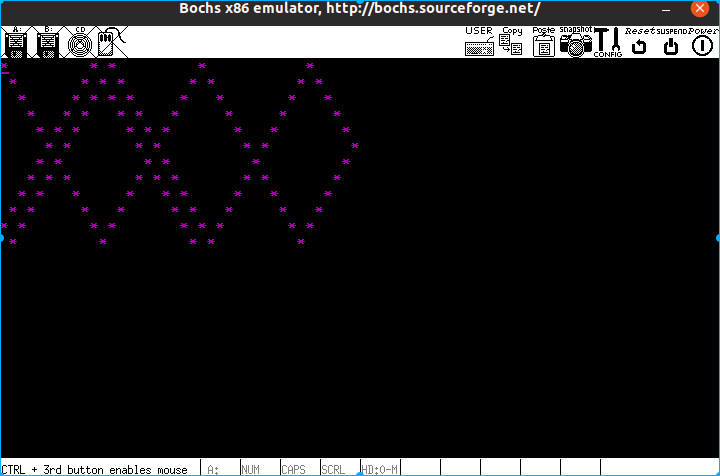
\includegraphics[width=15cm]{img/1.png}
		\bottomcaption{显示一个弹球弹幕}
	\end{figure}
	\begin{figure}[htbp]
		\centering
		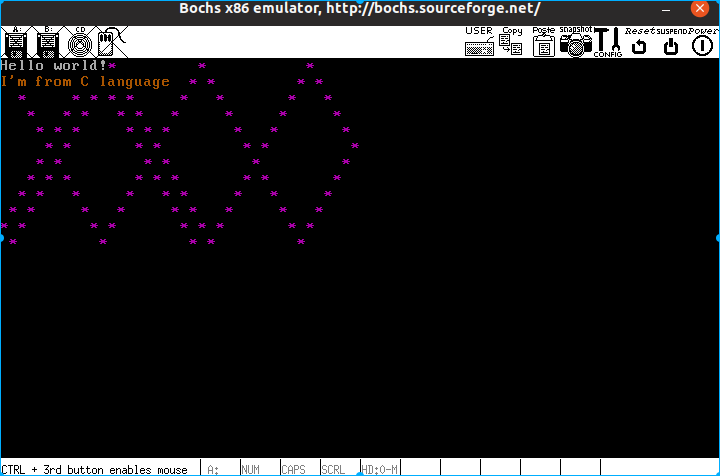
\includegraphics[width=15cm]{img/2.png}
		\bottomcaption{显示两个字符串}
	\end{figure}
	\begin{figure}[htbp]
		\centering
		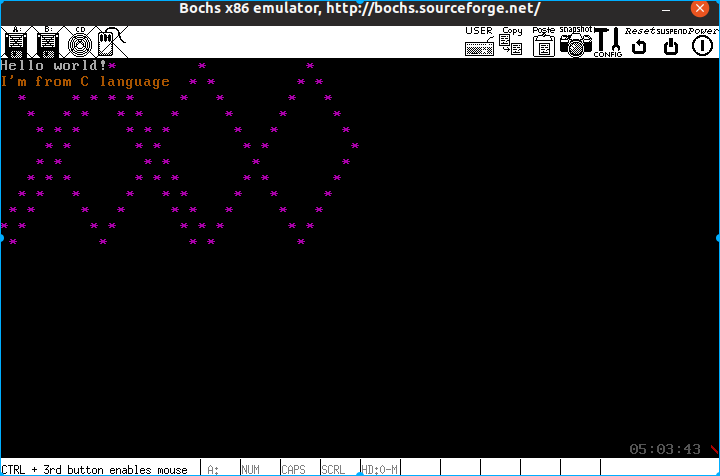
\includegraphics[width=15cm]{img/3.png}
		\bottomcaption{阻塞等待读入字符,此时右下角的时间开始显示}
	\end{figure}
	\begin{figure}[htbp]
		\centering
		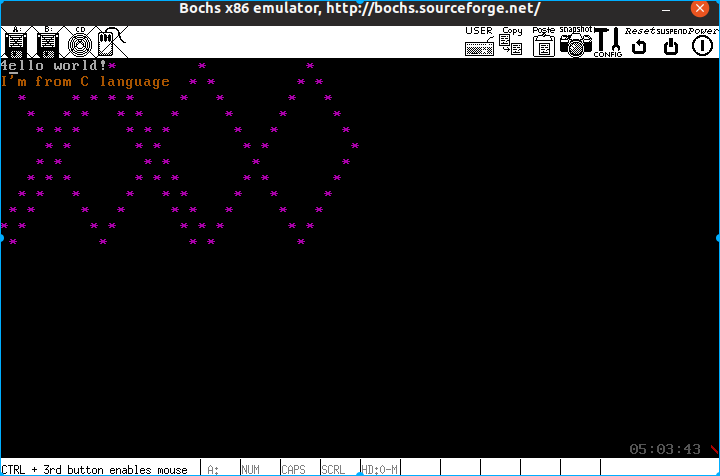
\includegraphics[width=15cm]{img/4.png}
		\bottomcaption{成功读入字符4,并显示在第一个位置}
	\end{figure}
	\begin{figure}[htbp]
		\centering
		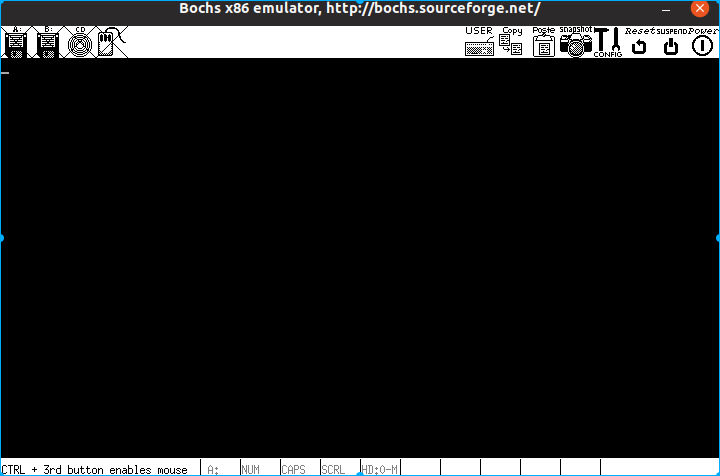
\includegraphics[width=15cm]{img/5.png}
		\bottomcaption{第一次调用清屏}
	\end{figure}
	\begin{figure}[htbp]
		\centering
		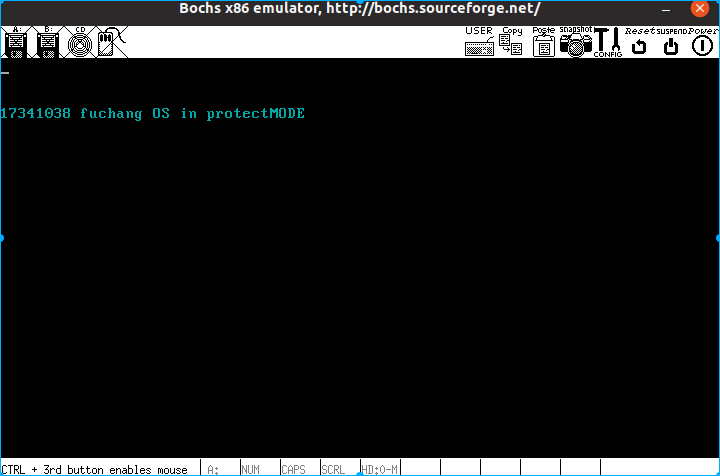
\includegraphics[width=15cm]{img/6.png}
		\bottomcaption{显示个人信息}
	\end{figure}
	\begin{figure}[htbp]
		\centering
		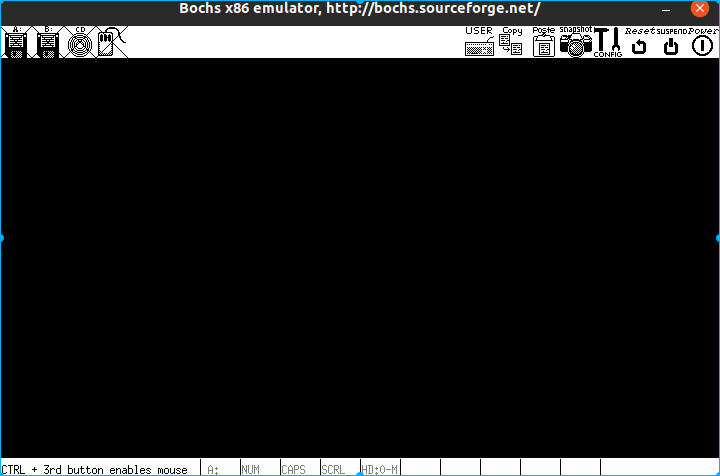
\includegraphics[width=15cm]{img/7.png}
		\bottomcaption{第二次清屏}
	\end{figure}
	\begin{figure}[htbp]
		\centering
		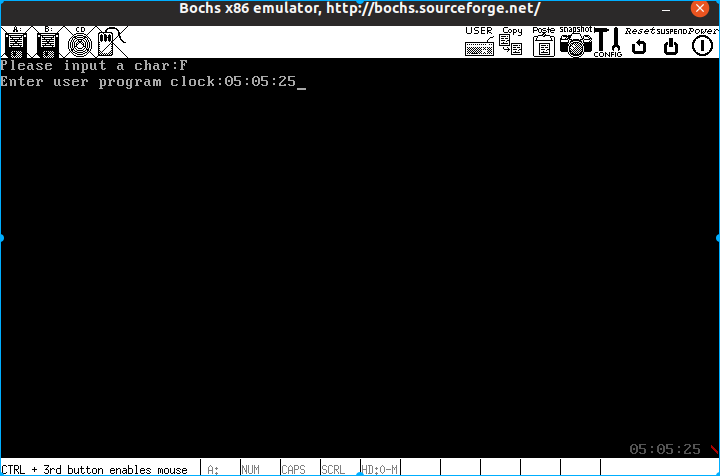
\includegraphics[width=15cm]{img/8.png}
		\bottomcaption{读入一个字符F并显示,接着便显示进入用户程序的时间,和右下角一致}
	\end{figure}
	\clearpage
			% \lstset{language=={[x86masm]Assembler}}
			% \begin{lstlisting}[language=={[x86masm]Assembler}keywordstyle=\color{blue!70},commentstyle=\color{red!50!green!50!blue!50},frame=shadowbox, rulesepcolor=\color{red!20!green!20!blue!20}]
			% \end{lstlisting}

			% \begin{lstlisting}[language={[ANSI]C},keywordstyle=\color{blue!70},commentstyle=\color{red!50!green!50!blue!50},frame=shadowbox, rulesepcolor=\color{red!20!green!20!blue!20}]
			% \end{lstlisting} 

	% \begin{figure}[htbp]
	% 	\centering
	% 	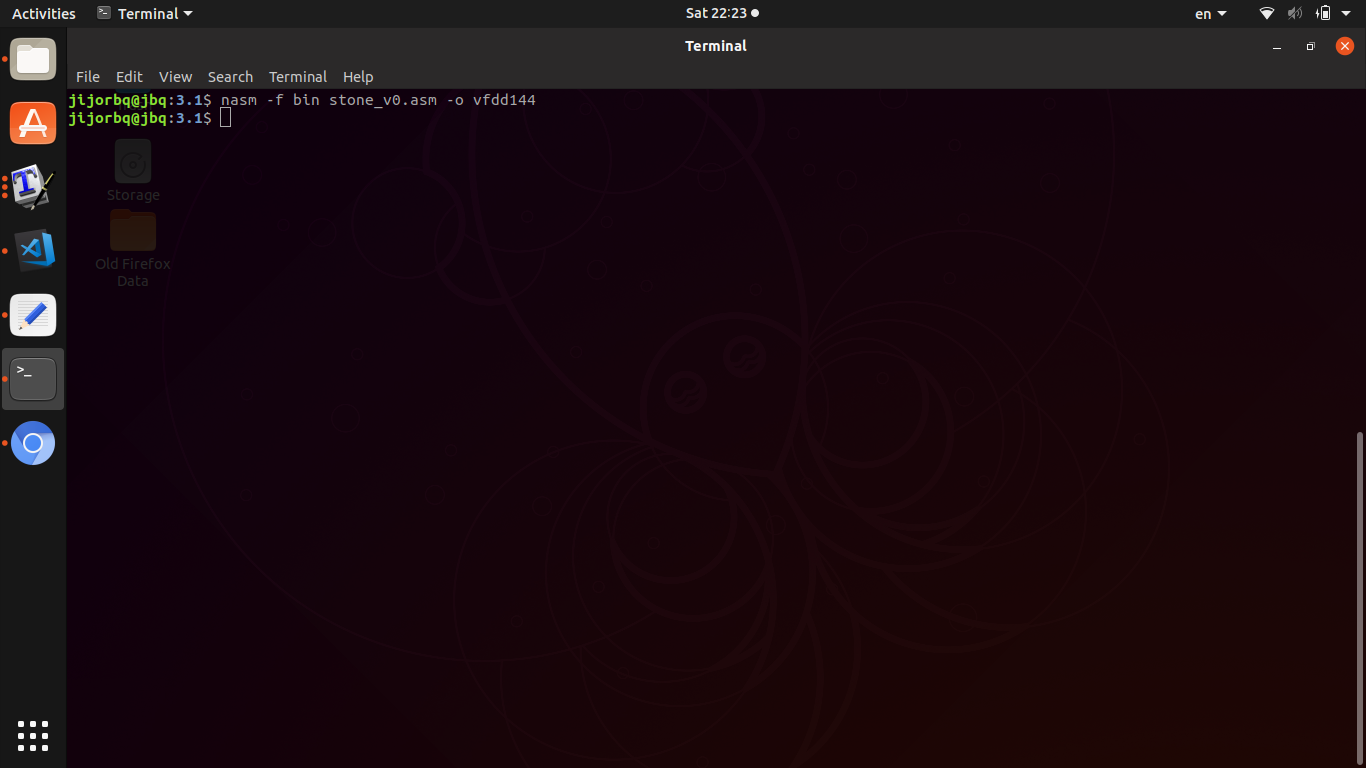
\includegraphics[width=10cm]{Screenshot from 2019-03-23 22-23-16.png}
	% 	\bottomcaption{终端直接执行}
	% \end{figure}
	% 终端直接执行:bochs -q -f bochsrc

	% \begin{figure}[htbp]
	% 	\centering
	% 	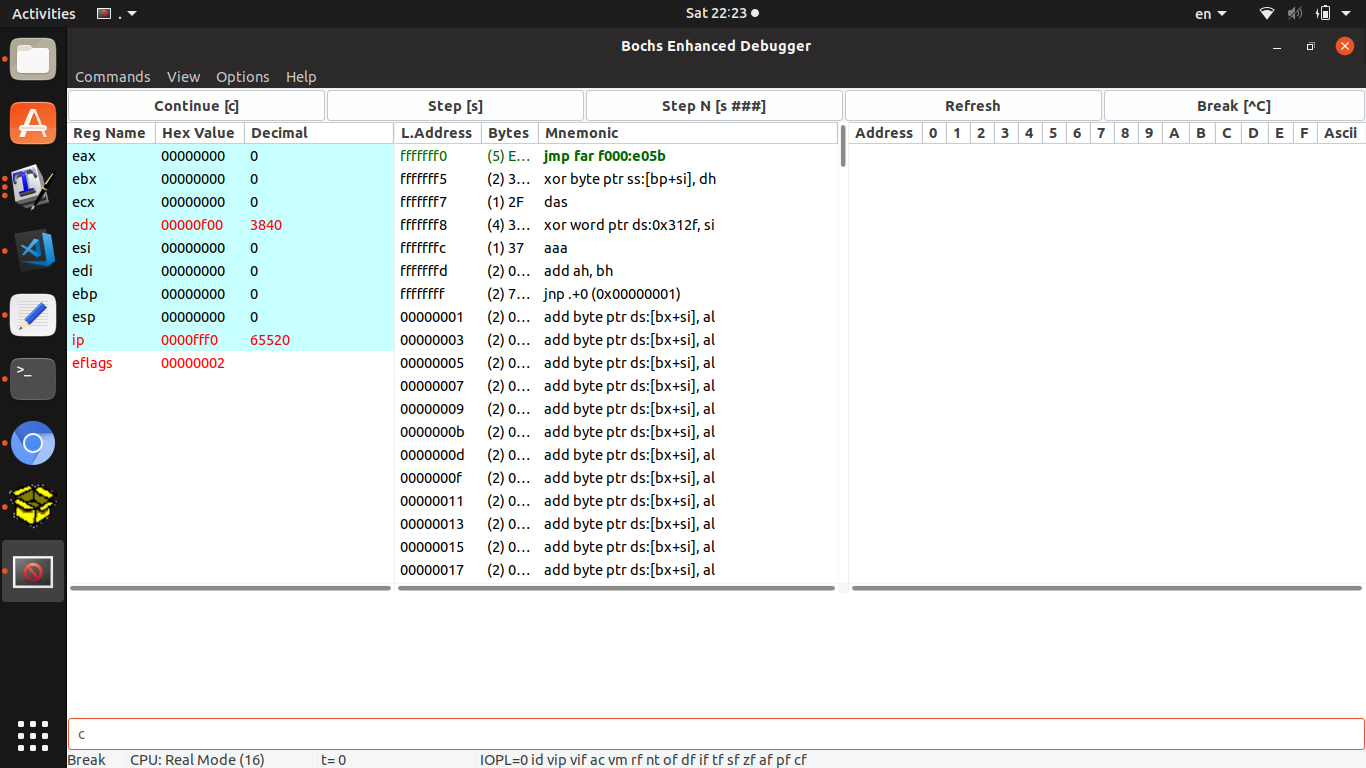
\includegraphics[width=10cm]{Screenshot from 2019-03-23 22-23-35.png}
	% 	\bottomcaption{打开bochs}
	% \end{figure}

	% 输入执行命令 "c"

	% \begin{figure}[htbp]
	% 	\centering
	% 	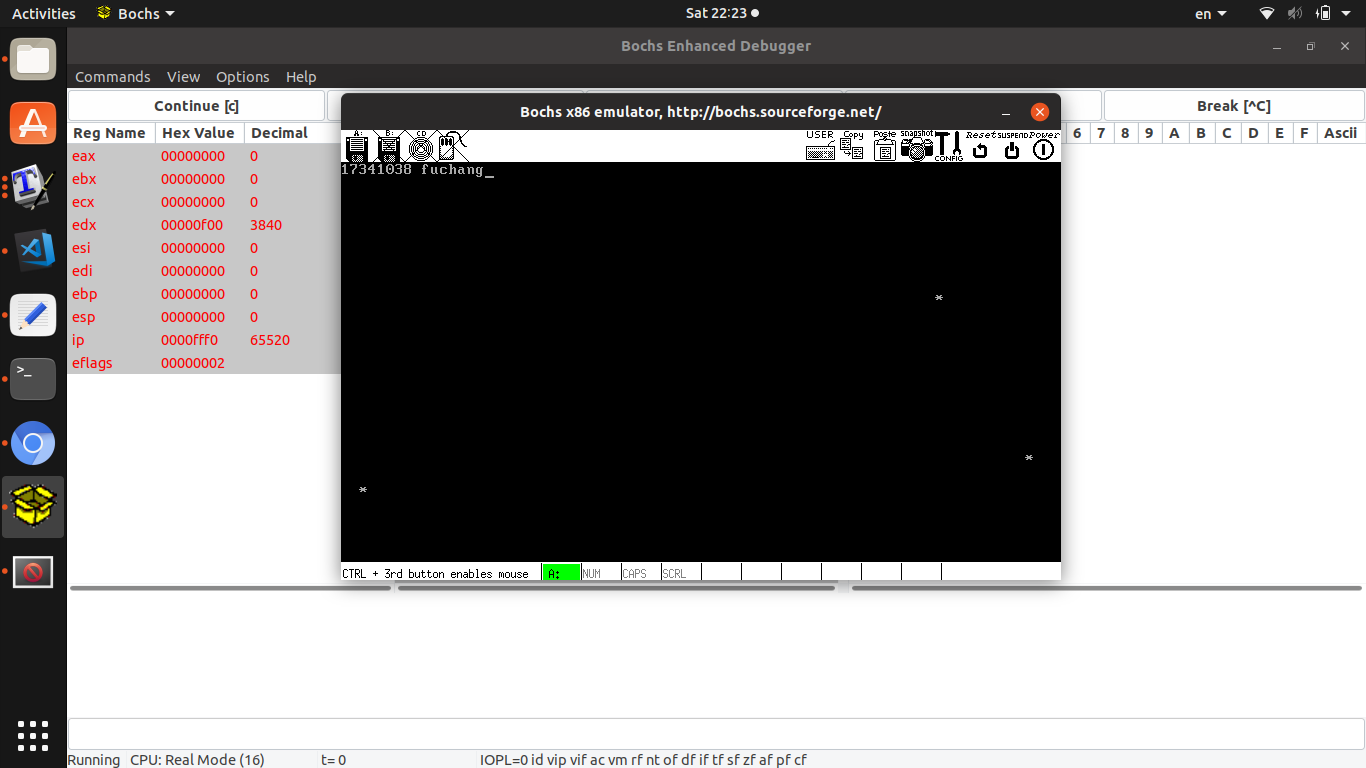
\includegraphics[width=10cm]{Screenshot from 2019-03-23 22-23-44.png}
	% 	\bottomcaption{显示}
	% \end{figure}




\section{实验总结}
	本次系统调用的实验是为以后实现多用户甚至多进程的模型做准备。日益增长的用户功能急需封装更多的系统调用。本次实验我掌握的通过软中断封装系统调用的方式实现了一些非常基本的IO函数\\
	\indent 尽管getchar还非常简陋,因为我还没能够支持shift输入转义字符。不过相比之前只能输出的程序,还是迈出了一大步\\
	\indent 因为系统调用是一个个添加的,并且做足了系统测试与模块测试,一些常见的不常见的bug总是很快地被调出来了。而且和以前不一样,由于贯彻了“先阅读手册和书籍”再写代码的教训,遇到问题总是能很快地摸清解决的方向并很快地找到解决方案,这相比起以前实验给我更有趣的体验。\\
	\indent 实验的不足还是有的,其中一个就是不能动态的确定被加载代码块的长度,这在以后代码模块动态变化很大的时候会造成隐患,这个问题应该在下一个实验得到解决。

\bibliographystyle{plain}
\bibliography{ref}

\clearpage



\end{document}
